\chapter{\label{profiling}Profiling}
In this chapter, we prove that the current state of the art bitcoin client does not scale well when the number of connected nodes is increased and is therefore not well suited for the use as a relay node. First, we show general measurement on various system performance indicators. After spotting the CPU to be the possible bottleneck, we perform an in depth analysis of the runtime behaviour of the two most heavy weight threads. This leads to the insight that the inter-thread communication is the bottleneck for scaling the bitcoin client.

\begin{figure}[!hbt]
\begin{center}
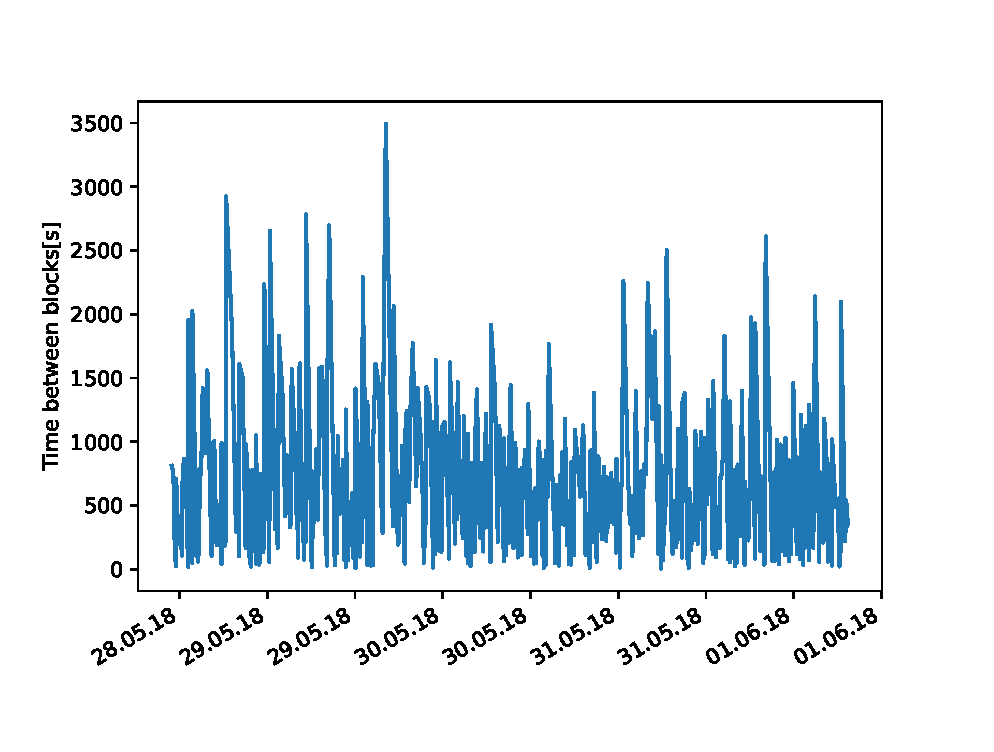
\includegraphics[width=0.5\textwidth]{block_dates}
\caption[Overview of the time between two successive bitcoin blocks.]{Overview of the time between two successive blocks. The time was measured for 650 blocks between 1.6.18 and 28.5.18 and is given in seconds on the y-axis. \label{figure:blockDates}}
\end{center}
\end{figure}

\section{Challenges \label{sec:measuringDifficutlies}}
Before we present the results, we discuss some challenges in measuring the performance of the bitcoin client. First, the bitcoin network is hard to observe in an isolated setting. The measurements were done with the bitcoin client connected to the bitcoin network. This means, that there are potentially large fluctuations in traffic. For example, as there is no fixed period for new blocks, it sometimes happens that there are no new blocks for 90 minutes. On the other hand, there are times when there are 4 new blocks in 10 minutes. To illustrate this, we plotted the time between two consecutive blocks in figure \ref{figure:blockDates}. To minimise the impact of such fluctuations, we designed the experiments to be long running and repeated them at least 3 times.\\
Second, the client does not allow an arbitrary amount of connections. The bitcoin client uses \textit{select} to query the sockets used for the connections to its peer. According to the linux manual page of \textit{select} \cite{select}, the total number of sockets that \textit{select} can handle is limited by FD\_SETSIZE which is hardcoded to 1024 on Linux distributions. Subtracting the 150 file descriptors that the client reserves for opening files and handling communication, it is possible to open 874 connections to peers. This behaviour could be changed by rewriting the logic of the bitcoin client to use \textit{poll} instead of \textit{select}, but this is not in the scope of this thesis. The consequence of this is that we were not able to generate an arbitrary load on the client during the experiments. Therefore, finding the bottleneck in the current state-of-the-art bitcoin client is hard.


\section{\label{profiling:setup}Methodology}
In this section, the general experimental setup and the tools used are presented. The actual experiments are described together with the results in section \ref{profiling:results}. 
\subsubsection{Device under test}
The experiments were run on two devices:
\begin{enumerate}
	\item Laptop with Intel dual Core i7 M620 CPU running at 2.67GHz with hyper-threading enabled. 4GB RAM. Running Debian Stretch. \newline This device is referred to as \textit{device 1}.
	\item Laptop with Intel dual Core i7 6600U CPU running at 2.60GHz with hyper-threading enabled. 20GB RAM. Running Ubuntu Xenial. \newline This device is referred to as \textit{device 2}.
\end{enumerate}
Note that \textit{device 2} has a more performant CPU and more memory than \textit{device 1}. 








\subsubsection{Client under test}
All experiments were performed with version 0.16 of the bitcoin client.\\
Only minor modifications were made to the client. First, the hardcoded connection limits were increased in net.h. 
\begin{PseudoCode}
	MAX_OUTBOUND_CONNECTIONS = 30
	MAX_ADDNODE_CONNECTIONS = 850
	DEFAULT_MAX_PEER_CONNECTIONS = 1000
\end{PseudoCode}
The values were chosen according to the limitations of the OS and the bitcoin client implementation (see section \ref{sec:measuringDifficutlies}).\\
For some experiments, it is necessary to connect two specific clients to each other. To guarantee that this connections are always established successfully, a minor change was made to always allow incoming connections from whitelisted peers. The following change was made in net.cpp:
\begin{diffCode}
@@ -1121,7 +1123,7 @@ void CConnman::AcceptConnection(const ListenSocket& hListenSocket) {
         return;
     }

-    if (nInbound >= nMaxInbound)
+    if (nInbound >= nMaxInbound && !whitelisted)
     {
         if (!AttemptToEvictConnection()) {
             // No connection to evict, disconnect the new connection
\end{diffCode}
Using the program \textit{top}, the priority of the bitcoin client process is increased to minimise the effect of background processes on the measurement.









\subsection{Measurement tools}
Various tools were used to measure the resources used by the bitcoin client. For reference, they are listed here.

\subsubsection{Ping client}
The \textit{ping client} is a modified version of the bitcoin client. This client will ignore most incoming messages and will send a bitcoin \textit{ping} message to the regular client every second. The \textit{ping client} only connects to the regular client and does not maintain or open other connections. The times when a \textit{ping} message is sent and when the \textit{pong} answers arrive are logged. Bitcoin clients by default send a \textit{ping} message every 120s. This time was reduced to one \textit{ping} per second. Note that the client does not send a \textit{ping}, if there is already a \textit{ping} request pending. Therefore, the actual period is defined as $\min\geschwungeneKlammern{1s,\mbox{RTT},\mbox{timemout}}$. The client does no other work. It does not accept other connections and does not ask for transactions or blocks. This keeps the \textit{ping client} lightweight. The exact changes can be seen in appendix \ref{appendix:pingClient}.\\
To make sure that the \textit{ping client} is able to connect to the bitcoin client, its ip was added to the whitelisted peers in the configuration of the client under test.

\subsubsection{gperftools}
\textit{gperftools}, short for great performance tools or google performance tools, was used to profile the CPU during runtime of the bitcoin client. \textit{gperftools} uses a stack sampling approach for profiling the CPU. A timer fires with a fixed frequency. When the timer fires, the profiler checks which function is currently executed by looking at the current stack frame. This approach leads to measurement inaccuracies, but it allows profiling with low overhead. The profiling time was set to multiple hours and the experiments were repeated multiple times to get statistically significant results. The exact times are given in the detailed experiment setups in section \ref{profiling:results}. \textit{gperftools} was chosen as a profiler because it is well suited for profiling multithreaded applications and produces little overhead. Note that in case of multithreaded profiling, the threads that should be profiled have to call ProfilerRegisterThread() after they are created. This will add a new timer for this thread. Configuration was done using environmental variables. The following settings were used:
\begin{PseudoCode}
	export CPUPROFILESIGNAL=12 			# signal used to start and stop profiling
	export CPUPROFILE=~/gproftools.prof 		# location to save the output profile to
	export CPUPROFILE_FREQUENCY=100 		# sampling frequency (samples/s)
	export CPUPROFILE_REALTIME=1 			# use the Linux interval timer
	export CPUPROFILE_TIMER_SIGNAL=34 		# use another timer signal not to 
							# interfer with SIGALARM
\end{PseudoCode}
\textit{gperftools} creates a profile in a binary format which can be translated to call graphs or that can be imported to kcachegrind/qcachegrind\cite{cachegrind}. These tools provide a graphical interface to navigate through the collected data. For more details, the documentation of the CPU profiler of \textit{gperftools} can be found in \cite{gperftools}.

\subsubsection{vmstat}
\textit{vmstat} is a Linux tool to report the usage of various system resources. \textit{vmstat} reads these information from the /proc filesystem. It is used, because it shows a broad overview of many system parameters such as swap usage, memory usage, disk I/O, interrupt frequency, frequency of context switches, the CPU usage and the I/O wait time. Using \textit{vmstat}, all information is in a common place which makes the analysis easier. More information can be found in the Linux manual page in \cite{vmstat}.

\subsubsection{top/ps}
\textit{top} and \textit{ps} are standard Linux tool to get realtime information about the current resource usage. They are able to show per thread CPU usage and the total amount of memory used. \textit{top} was used because of its ability to continuously measure. \textit{ps} was used because it the output can be formatted more easily, which helps for the analysis of the experiments. Otherwise, the two programs can be used interchangeably. More information about \textit{top} and \textit{ps} can be found in the Linux manual pages in \cite{top} and \cite{ps}. 




\section{\label{profiling:results}Experiments}
In this section, a series of 4 experiments is presented. First, we measure the performance of a client that is connected to an increasing numer of peers. After experiencing a performance degeneration in this experiment, a second experiment is done which shows the resource usage of the bitcoin client when it is connected to a maximum of 860 peers. The last two experiments analyse the increased CPU usage of the client and show that the inter-thread communication is limiting the scaling of the currently used standard client. In the following, the reasoning behind the experiments and the exact setups are explained and the results are presented and explained.

\begin{figure}[!bt]
\begin{center}
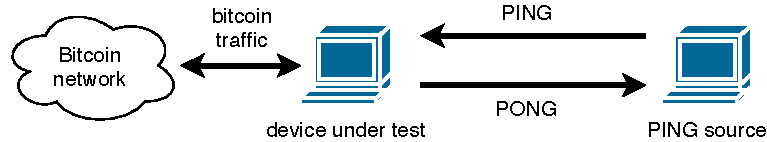
\includegraphics[width=0.8\textwidth]{Figures/pingmachine.pdf}
\caption[Test setup for the performance degeneration test]{Test setup for the performance degeneration test. The \textit{ping client} sends a \textit{ping} every second. The device under test replies with a \textit{pong} message. The times when a \textit{ping} is sent or a \textit{pong} is received are logged at the \textit{ping client}. During the test, the client receives regular bitcoin messages from its peers over the bitcoin network. \label{figure:pingmachine}}
\end{center}
\end{figure}

\subsection{Performance degeneration \label{sec:perf_degen}}
The goal of the first experiment is to show that the performance of the bitcoin client degenerates when connecting to many peers. The load on the client is dependent on the current state of the bitcoin network and the peer activity in general (see section \ref{sec:measuringDifficutlies}). Furthermore, the load is dependent on the time. For example, a higher load is expected when a block has to be verified.\\ 
There are 2 network parameters commonly measured to make assumptions about networks. The first of them is throughput. The intention would be that the bitcoin client is not able to process the data fast enough when connected to many peers and would drop packet or would throttle the amount of messages sent. As argued in section \ref{sec:measuringDifficutlies}, it was not possible to bring the client to its limits and therefore we could not observe any packet drops or intentional message throttling which makes the use of the throughput as performance indicator difficult to measure and to interpret. The other common performance indicator is the latency. We measured the RTT of a client connected to the bitcoin client under test. The expected result is an increasing delay at the client when it is connected to an increasing number of peers. To measure the performance of the client, the RTT of a \textit{ping}/\textit{pong} exchange was measured using the \textit{ping client}. According to the bitcoin protocol, upon the arrival of a \textit{ping} message, a client must respond with a \textit{pong} message\cite{bitcoinNetworkProtocol}. 
\subsubsection{Setup}
The \textit{ping client} runs on the same host as the software under test. The setup is illustrated in figure \ref{figure:pingmachine}. The experiment was conducted as follows:
\begin{itemize}
	\item The bitcoin client is started.
	\item The \textit{ping client} is started.
	\item Iterate over the following desired connection levels: 30, 100, 300, 500, 700, 860 and for each level do the following:
	\begin{itemize}
	\item Establish new connections until the desired connection level is reached.
	\item Wait for 15 minutes to assure that the client is in a steady state.
	\item The measurement starts. For 1 hour, the actual number of connected peers is logged and new connections are established, if the connection count drops below the desired level. The logged data is used to match the logs from the \textit{ping client} to a connection count level and to verify that the desired connection count matches the actual number of open connections.  
	\end{itemize}
\end{itemize}
We run the experiment 3 times on both devices. This means that every of the discrete connection levels in the experiment was measured for 3h per device.\\


\subsubsection{Results}
The results of this experiment are listed in table \ref{tab:performance_degeneration}. We are interested in the change of the measured RTT.  In figure \ref{fig:rtt}, the data is plotted. The plot shows the increase of the delay when additional connections are established at the client. We note that after 300 connections, the additional overhead per added connection gets larger. We assume that the increase is smaller for \textit{device 2}, because the device has better stats. The results show that the RTT is dependant on the number of connections which is a clear sign of bad scaling properties of the bitcoin client.\\
%Incoming messages at the client can be split into two categories: The first category contains all messages that is dependant on the number of connections, e.g. PING messages or advertisements of transactions. Messages that are independent of the number of connected peers belong to the second category. Examples for messages in this category are incoming transactions or blocks. Generally, messages of the second category cause larger overhead at the receiving client, because transactions and blocks need verification while messages from the first category can be replied without large overhead. Because of this, we would not expect the 

\begin{table}[tbp]
\begin{center}\begin{minipage}{\textwidth}
\begin{center}
\begin{tabular}{r | r |r}
\textbf{Number of connections} & \textbf{RTT \textit{device 1} [$\mu s$]} & \textbf{RTT \textit{device 1} [$\mu s$]} \\
\hline
30 & 8'198		& 3'754 \\
100 & 7'151 	& 5'630 \\
300 & 26'420 	& 8'930 \\
500 & 81'797 	& 20'794 \\
700 & 174'920 	& 30'482 \\
860 & 187'246 	& 40'246 \\
\end{tabular}
\end{center}
\end{minipage}
\caption[RTT measurements of the bitcoin client.]{RTT measurements of the bitcoin client. The RTT of a \textit{ping}/\textit{pong} exchange with the bitcoin client is measured for different numbers of peer connections.}
\label{tab:performance_degeneration}
\end{center}
\end{table}

\begin{figure}[!bt]
\begin{center}
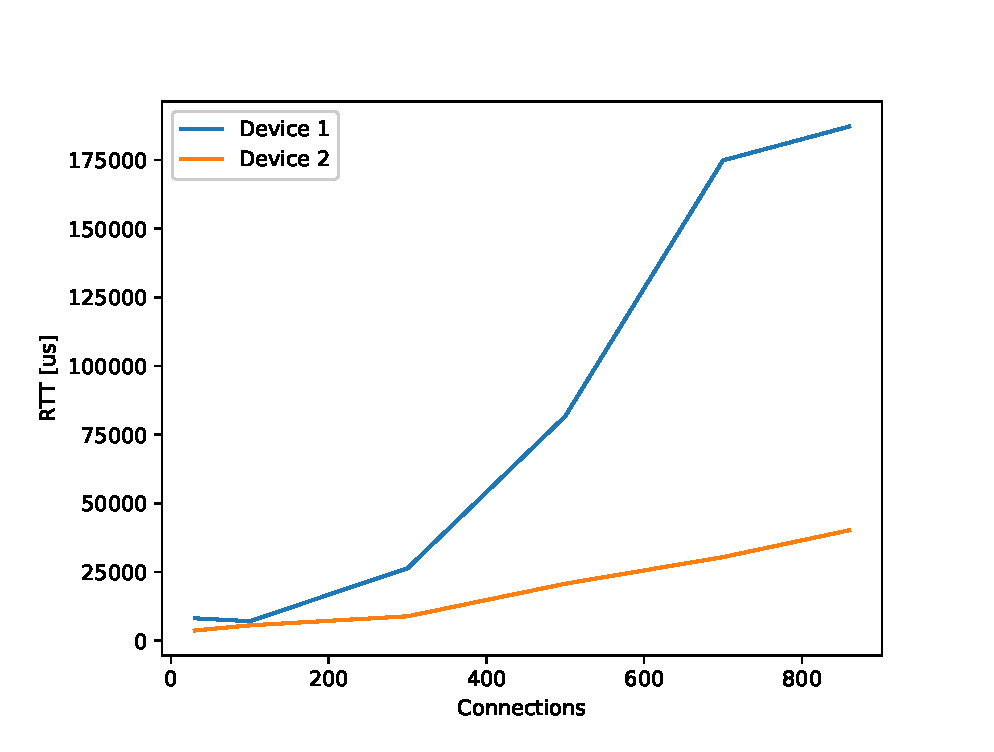
\includegraphics[width=0.7\textwidth]{rtt}
\caption[RTT measurements of the bitcoin client.]{This figure shows the measured RTT of a ping/pong message exchange when the client under test is connected to an increasing number of peers. We see that the delay is increasing with the number of connections. After around 300 connections we see a larger increase in the delay for both devices.}
\label{fig:rtt}
\end{center}
\end{figure}




\subsection{General Resource Usage \label{sec:generalResources}}
We have seen that the performance of the client becomes worse when more connections are added. To find the limiting factor on the performance, we do another experiment and measure various system parameters. CPU, I/O, Swap and Memory usage were measured. 
\subsubsection{Setup}
\begin{itemize}
	\item The bitcoin client is started.
	\item Iterate over the following desired connection levels: 30, 100, 300, 500, 700, 860. For each, do the following:
	\begin{itemize}
	\item Establish new connections until the desired connection level is reached.
	\item Wait for 15 minutes to assure that the client is in a steady state.
	\item The measurement starts. For 1 hour, the actual number of connected peers is logged and new connections are established, if the connection count drops below the desired level.\textit{vmstat} is used to measure the CPU usage in user and kernel space, the number of context switches, the I/O wait time, the amount of free memory, the amount of swap used and the amount of kernel buffer space used. One measurement is taken every 5 seconds.
	\end{itemize}
\end{itemize}
We run the experiment 3 times on both devices. This means that every of the discrete connection levels in the experiment was measured for 3h per device.\\
\subsubsection{Results}




An overview of the results can be found in table \ref{tab:recource_usage}. For the CPU measurements we note, that the CPU usage in both devices increases, while the idle time of the CPU decreases. The absolute values for the total CPU usage at 860 connections reported by \textit{vmstat} (mean value over the 3h of experiment) are 52\% and 47\% for \textit{device 1} and \textit{device 2} respectively. \textit{vmstat} gives the values in respect to the total computing power. However, it is not clear if this load is distributed evenly across the 4 virtual CPU cores both devices have. To check this, the experiment in section \ref{sec:threading} is done. \\
 We observe many context switches. Using \textit{strace}, we see that approximately 90\% of the system calls are calls to \textit{futex}. According to Franke et Al. in \cite{franke2002fuss}, the call to \textit{futex} is used for fast thread synchronisation.\\
 When looking at the I/O measurements, we note that disk reads and disk writes do not seem to be the bottleneck as the measurements at 860 nodes show a similar amount of disk reads/writes as the measurement at 30 nodes. The same is true for the I/O wait measurement which measures the time a process has to wait for I/O devices in general. We see an increase in interrupts. This is expected as the network interface does receive more messages and will therefore produce more interrupts.\\
 From the data, it is clear that swapping is not causing the performance degeneration. This is also clear as the memory usage peaks at around 35\% and there is no need for excessive swapping. Also the buffer space used to store kernel space object does not seem to run out.\\
 With these result, I/O and memory bottlenecks can be ruled out. We noted, that the CPU usage only goes up to around 50\%. Next, we will check how the workload is distributed over the cores. This will allow us to pinpoint the bottleneck to the CPU or rule this factor out as well.










\subsection{Per thread CPU usage measurement \label{sec:threading}}
We noticed that the CPU usage is increasing. However, the overall CPU usage only goes up to approximately 50\%. As the client is multithreaded, we would expect the load to spread across all 4 virtual cores. However, if the load is not distributed evenly, it could be the case that 1 or 2 cores run at 100\%. We do an additional experiment, in order to show that which part of the system is using most CPU time and that the load is not spread evenly across the cores. For this, the CPU usage was measured on a per-thread basis.\\

\subsubsection{Setup}
\begin{itemize}
	\item The bitcoin client is started.
	\item Iterate over the following desired connection levels: 30, 100, 300, 500, 700, 860. For each do the following:
	\begin{itemize}
	\item Establish new connections until the desired connection level is reached.
	\item Wait for 15 minutes to assure that the client is in a steady state.
	\item The measurement starts. For 1 hour, the actual number of connected peers is logged and new connections are established, if the connection count drops below the desired level. \textit{ps} is used with the -L command line option which shows the per thread CPU and memory usage. Measurements are taken every second.
	\end{itemize}
\end{itemize}
We run the experiment 3 times on \textit{device 1} and \textit{device 2}. This means that every of the discrete connection levels in the experiment was measured for 3h per device.\\
\subsubsection{Results}
The results of the experiment are plotted in figure \ref{fig:threads}. The result looks similar for both devices, thus only the results of \textit{device 1} are shown.
We see that the SocketHandler thread (bitcoin-net) and MessageHandler thread (bitcoin-msghand) are responsible for most of the CPU usage. At 860 connections, these two threads are using about 90\% of CPU time. Again, if the system was loaded, we would expect the CPU time for at least one of these threads to go up to 100\%.\\
The CPU time reported by top is a mean over a certain period of time. We perform a variant of the experiment with additional resolution to get a more fine grained view of the CPU usage of the SocketHandler thread and the MessageHandler thread. For this, we increase the sampling frequency and keep track of how many times the CPU time goes up to 99.9\%.
\subsubsection{Setup 2}
\begin{itemize}
	\item The bitcoin client is started.
	\item Connection setup requests are sent to the client using the command line interface. The requests are sent at a fixed frequency of 8 connections per second. During the connection establishment, the CPU usage is measured every 100ms. Additionally, the number of established connections is logged.
	\item When the client reaches 860 let it run for another minute and then stop.
\end{itemize}
The experiment was run 3 times on \textit{device 1}.\\
\subsubsection{Results 2}
 We see in figure \ref{subfigure:bursts}, that for the SocketHandler thread (bitcoin-net) the number of these "bursts" (moments when the CPU usage is above 99.9\%) of CPU usage increases with an increasing number of connections. Interestingly, we observe that starting from about 400 connections the amount of these "bursts" decreases for the MessageHandler thread at about the same rate at which it is increasing for the SocketHandler thread. The reason for this becomes clearer after the next experiment.\\


\begin{figure}[!pbt]
\begin{center}
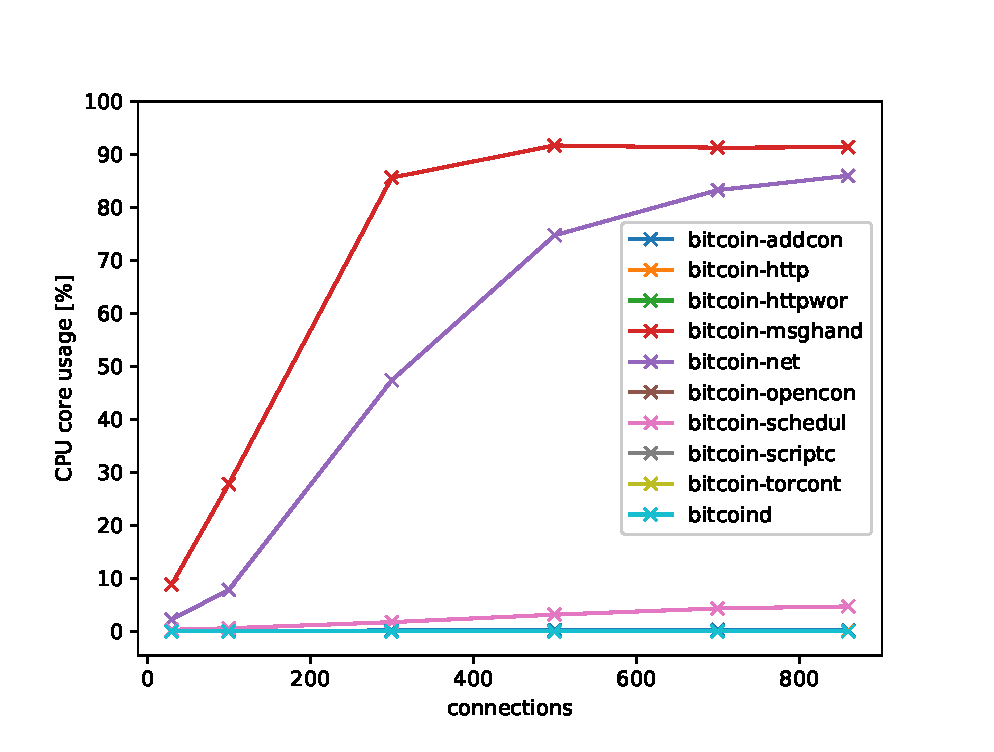
\includegraphics[width=0.7\textwidth]{threads}
\caption[Per thread CPU usage]{CPU usage of the individual threads of the bitcoin client when connected to different numbers of peers. The only two threads using a lot of CPU time are the bitcoin-net and bitcoin-msghand threads. The other threads use less than 5\% CPU time.}
\label{fig:threads}
\end{center}
\end{figure}

\begin{figure}[!pbt]
\begin{center}
\begin{subfigure}[t]{0.49\textwidth}
	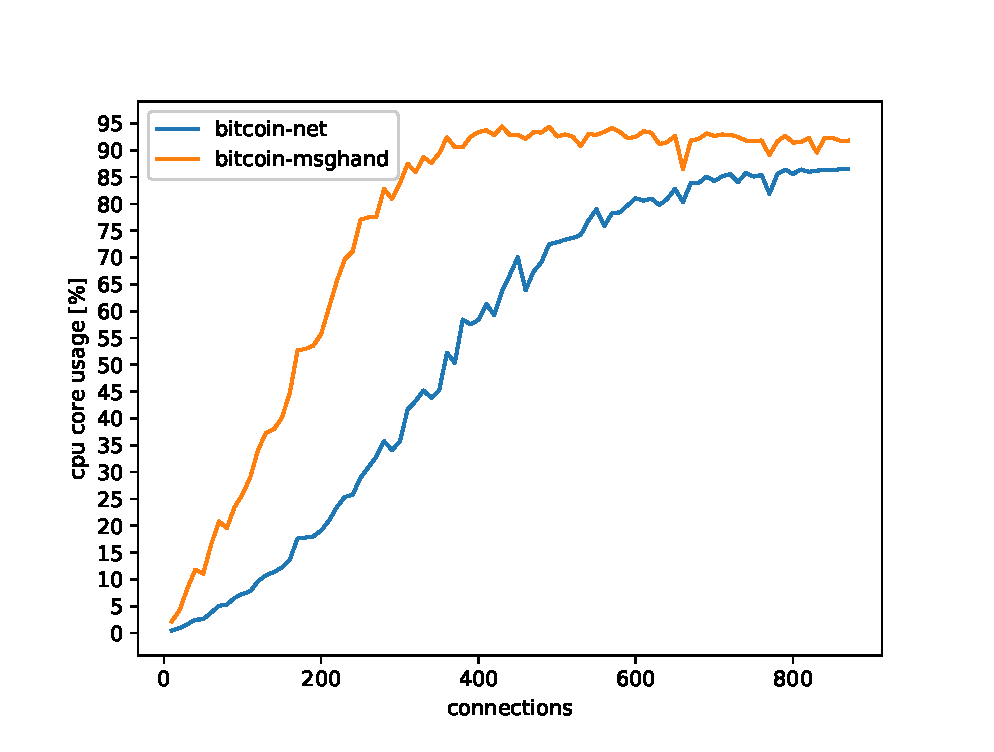
\includegraphics[width=\textwidth]{cpuUsage}
  \subcaption[CPU usage of the two most heavy weight threads.]{CPU usage of the MessageHandler and the SocketHandler as a function of the number of connected peers. We see that both threads increase to about 90\% CPU time. After that, the CPU time used does not increase anymore when adding additional connections.}
  \label{subfigure:cpuUsage}
\end{subfigure}
\hfill
\begin{subfigure}[t]{0.49\textwidth}
	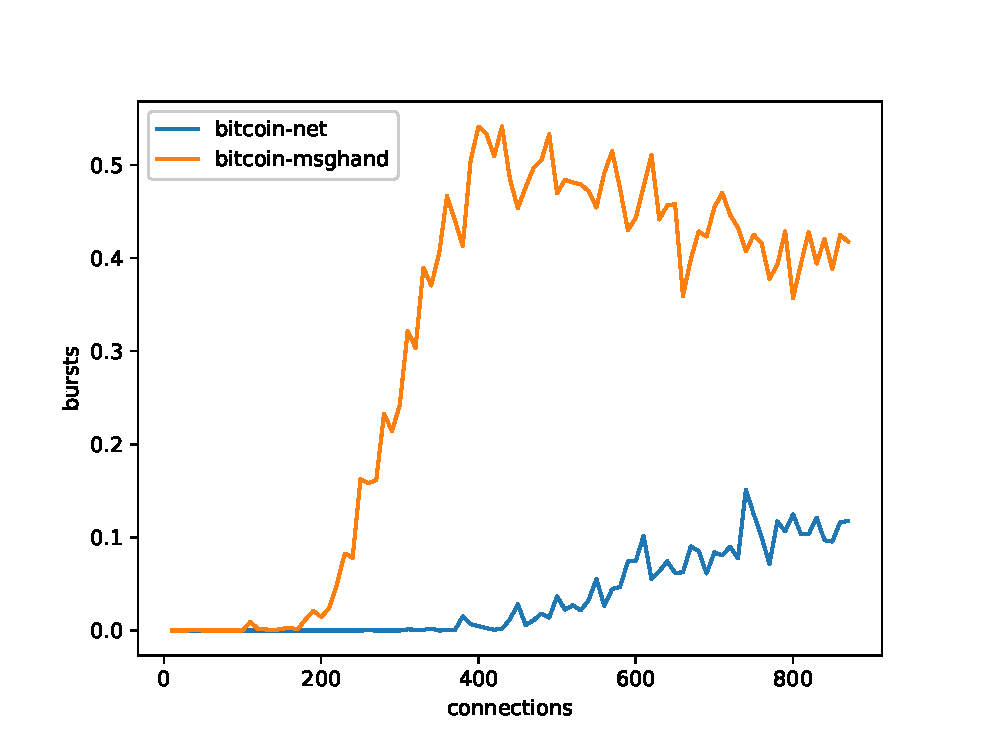
\includegraphics[width=\textwidth]{bursts}
  \subcaption{Ratio between the measurement points above and below 99.9\% CPU usage. By looking at the amount of time the threads are using more than 99.9\% CPU time, we get a more fine grained view over the trend of the CPU usage of the threads. At around 400 connections, we see that the CPU time for the bitcoin-msghand thread starts to decrease while the CPU time of the bitcoin-net thread increases.}
  \label{subfigure:bursts}
\end{subfigure}
\caption[Detailed CPU usage of the MessageHandler and the SocketHandler threads]{Detailed CPU usage of the MessageHandler and the SocketHandler threads.}
\label{fig:burst}
\end{center}
\end{figure}




\subsection{Thread work analysis \label{sec:workAnalysis}}
By now, we have strong evidence that the CPU usage is linked to the bottleneck for the scaling of the bitcoin client on our test devices.
The following experiment shows the difference in the workload distribution of the tasks that are performed by the SocketHandler thread and the MessageHandler thread under different load. 
\subsubsection{Setup}
The measurement is done using \textit{gperftools}. The experiment is conducted on \textit{device 1}. The test setup is the following:
\begin{itemize}
	\item The bitcoin client is started.
	\item Iterate over the following desired connection levels: 30, 400, 860. For each level do the following:
	\begin{itemize}
	\item Establish new connections until the desired connection level is reached.
	\item Wait 15 minutes to guarantee a normal mode of operation
	\item Profile the CPU usage using gperftools for 4 hours. For this, \textit{ProfilerRegisterThread()} was compiled in at the start of the SocketHandler thread and the MessageHandler thread to enable individual timers for these two threads.
\end{itemize}
\end{itemize}
This experiment was repeated 3 times. This leads to a total of 12h measurement for 30, 400 and 860 connections, each.

\subsubsection{SocketHandler thread}
We focus on the three function calls that use the most CPU time when 30 connections are established. Therefore, the results presented will not sum up to 100\%. An overview of these functions and what they are used for can be found below.
\begin{itemize}
	\item \textbf{\textit{CriticalBlock::CCriticalBlock}:} Wrapper that is used for thread synchronisation. Makes the current scope a critical section. A std::recursive\_mutex lock is acquired that is automatically released when the scope ends.
	\item \textbf{\textit{\_\_select}:} In the context of the bitcoin client, \textit{\_\_select} checks for incoming packets and the availability of sending messages by checking the TCP sockets of all connected clients.
	\item \textbf{\textit{CThreadInterrupt::sleep\_for}:} The calling thread waits until the timeout exceeds or the thread is waked by another thread. This roughly translates to "there is nothing to receive or send".
\end{itemize}
The result of the experiment can be seen in table \ref{tab:task_mix_socket}. Note that the time spent in \textit{CThreadInterrupt::sleep\_for} is a lot smaller at 860 connections than at 30 connections which shows that the thread has to do significantly more work. Intuitively, one would expect the \textit{\_\_select} call to grow with an increasing number of connections. Note that the results are relative numbers and only show the proportions of the function calls. This means, that the actual time spent in the \textit{\_\_select} function can be (and actually is) higher when connected to 860 peers than when connected to 30 peers, because the thread also uses more CPU time in total.\\
The main observation here is, that when connected to 860 peers, most of the CPU time used by the thread is used to handle the critical sections which are used to communicate with other threads (especially with the MessageHandler thread). 

\begin{table}[!htbp]
\begin{center}
\begin{minipage}{\textwidth}
\begin{center}
\begin{tabular}{l|r|r|r}
\textbf{Function} & \textbf{30 conn. [\%]} & \textbf{400 conn. [\%]} & \textbf{860 conn. [\%]} \\
\hline
\small CriticalBlock::CCriticalBlock & 1.7 & 38.0 & 64.9\\
\small \_\_select & 16.1 & 10.7 & 4.4 \\
\small CThreadInterrupt::sleep\_for & 80.8 & 37.5 & 3.7 \\
\end{tabular}
\end{center}
\end{minipage}
\end{center}
\caption[Difference in CPU time of 3 selected functions of the SocketHandler thread.]{Difference in CPU time of 3 selected functions of the SocketHandler thread when running with 30, 400 and 860 clients. The unit is the percentage of the cumulated CPU time of the function and all its subfunctions in respect to the total CPU time of the thread.}
\label{tab:task_mix_socket}
\end{table}



\subsubsection{MessageHandler thread}
We focus on the three function calls that use the most CPU time when 30 connections are established. Additionally, we focus on the function \textit{CriticalBlock::CCriticalBlock} because it is using a high amount of CPU time when the client is connected to 860 peers. The results do not sum up to 100\% because the some functions are filtered out. Also, \textit{CriticalBlock::CCriticalBlock} is called by various functions in the MessageHandler thread.
\begin{itemize}
	\item \textbf{\textit{PeerLogicValidation::ProcessMessages}:} This function handles the message according to the message type. This includes the verification of transactions and blocks, the request of new blocks and transactions and the assembly of responses to the peer. If possible, the messages are sent immediately.
	\item \textbf{\textit{PeerLogicValidation::SendMessages}:} Assemble messages that are not a direct response to incoming messages. This includes for example periodic \textit{ping} messages, own transactions or advertisements. If possible, the messages are sent immediately.
	\item \textbf{\textit{std::condition\_variable::wait\_until}:} The calling thread waits until the timeout exceeds or the thread is waked by another thread. This roughly translates to "there are no new messages to process".
	\item \textbf{\textit{CriticalBlock::CCriticalBlock}:} Wrapper that is used for thread synchronisation. Makes the current scope a critical section. A \textit{std::recursive\_mutex} lock is acquired that is automatically released when the scope ends.
\end{itemize}
The results of the experiment are summarized in table \ref{tab:task_mix_message}. As expected, the functions \textit{PeerLogicValidation::SendMessages} and \textit{PeerLogicValidation::ProcessMessages} increase with the number of connections. This is because more connections lead to more incoming and outgoing messages. From the decrease of \textit{std::condition\_variable::wait\_until}, we see that the thread spends less time idle. Like with the SocketHandler thread, we observe a clear increase of the overhead of thread synchronising tasks. This increase seems to be lower after 400 connections.

% also mention last experiment

\begin{table}[htbp]
\begin{center}
\begin{minipage}{\textwidth}
\begin{center}
\begin{tabular}{l|r|r|r}
\textbf{Function} & \textbf{30 conn. [\%]} & \textbf{400 conn. [\%]} & \textbf{860 conn. [\%]} \\
\hline
\small PeerLogicValidation::ProcessMessages 	& 2.6  & 20.5  	& 31.4\\
\small PeerLogicValidation::SendMessages 		& 8.5  & 66.7	& 66.3 \\
\small std::condition\_variable::wait\_until 	& 88.7 & 10.4	& 1.3 \\
\hline
\small CriticalBlock::CCriticalBlock 			& 1.5 & 30.3 	& 36.5 \\
\end{tabular}
\end{center}
\end{minipage}
\end{center}
\caption[Difference in CPU time of 4 selected functions of the MessageHandler thread.]{Difference in CPU time of 4 selected functions of the MessageHandler thread when running with 30, 400 and 860 clients. Note that the function \textit{CriticalBlock::CCriticalBlock} is not entirely called directly by the main routine of the thread but also include calls from subfunctions of the main routine of the thread. The unit is the percentage of the cumulated CPU time of the function and all its subfunctions in respect to the total computation time of the thread.}
\label{tab:task_mix_message}
\end{table}


\subsubsection{Interpretation}
From the data we collected we can see the following: 
First, we see that both heavy weight threads (MessageHandler and SocketHandler thread) spend less time idle while both coming near the limit of 100\% CPU core time. 
Second, we see that both threads use an increasing amount of CPU time for handling the acquiring and freeing of mutex locks. The current implementation of the bitcoin client uses recursive mutexes from the standard library to protect shared resources. Gautham et al. show in \cite{gautham2012implications} that the use of mutexes does not scale when handling many small critical sections. The current implementation of the bitcoin client writes every message into a CNode at least once which will lead to an increasing amount of lock/unlock operations when the number of connections is increased. 
The next observation is that for the MessageHandler thread, the amount of time spent in CriticalBlock::CCriticalBlock is almost stagnant between 400 connections and 860 connections. At the same time, we observed in the experiment in section \ref{sec:threading} that the CPU usage for the MessageHandler decreases after 400 connections. Together, these two observations lead us to the conclusion that CPU usage is not the bottleneck of the scaling of the bitcoin client, but the inter-thread communication. The increased amount of context switches due to calls to \textit{futex} that we have observed in section \ref{sec:generalResources} supports this hypothesis.


%\begin{table}[htbp]
%\begin{center}
%\begin{minipage}{\textwidth}
%\begin{center}
%\begin{tabular}{l|l|r|r|r|r|r|r }
%\textbf{category} & \textbf{Parameter} & \textbf{30} & \textbf{100} & \textbf{300} & \textbf{500} & \textbf{700} & \textbf{860} \\
%\hline
%CPU    & User & 100 & 191 & 555 & 689 & 726 & 743\\
%       & Sys & 100 & 151 & 442 & 666 & 718 & 742\\
%   & Idle & 100 & 94 & 66 & 55 & 53 & 52 \\
%   & Context switches & 100 & 316 & 2507 & 3934 & 4145 & 4195 \\
%\hline
%I/O    & Interrupts & 100 & 134 & 319 & 447 & 522 & 571 \\
%   & Disk reads & 100 & 40 & 31 & 40 & 97 & 89\\
%   & Disk writes & 100 & 40 & 48 & 55 & 61 & 65\\
%   & I/O wait & 100 & 45 & 35 & 39 & 49 & 46 \\
%\hline
%Swap & Swap & 100 & 100 & 100 & 100 & 100 & 100\\
%\hline
%Memory & Free memory & 100 & 100 & 200 & 241 & 277 & 408\\
%   & used Buffer space & 100 & 100 & 69 & 54 & 34 & 44\\
%\end{tabular}
%\subcaption{Results of \textit{device 1}}
%\vspace{5mm}
%\end{center}
%\end{minipage}
%\begin{minipage}{\textwidth}
%\begin{center}
%\begin{tabular}{l|l|r|r|r|r|r|r }
%\textbf{category} & \textbf{Parameter} & \textbf{30} & \textbf{100} & \textbf{300} & \textbf{500} & \textbf{700} & \textbf{860} \\
%\hline
%CPU    & User & 100 & 168 & 320 & 417 & 449 & 456\\
%       & Sys & 100 & 147 & 290 & 497 & 624 & 659\\
%   & Idle & 100 & 94 & 77 & 66 & 61 & 60 \\
%   & Context switches & 100 & 460 & 5208 & 10355 & 12817 & 13247 \\
%\hline
%I/O    & Interrupts & 100 & 161 & 736 & 1346 & 1679 & 1779 \\
%   & Disk reads & 100 & 32 & 2856 & 146 & 122 & 174\\
%   & Disk writes & 100 & 84 & 131 & 180 & 220 & 261\\
%   & I/O wait   & 100 & 100     & 100     & 100     & 100     & 100\\
%\hline
%Swap & Swap & 100 & 100     & 100     & 100     & 100     & 100 \\
%\hline
%Memory & Free memory & 100 & 82 & 66 & 51 & 37 & 32\\
%   & used Buffer space & 100  &  100 &   100  &  100 & 98 & 83\\
%\end{tabular}
%\subcaption{Results of \textit{device 2}}
%\end{center}
%\end{minipage}
%\caption{Resource usage measurement on both test devices for 6 connection count levels which were each measured for 3 hours. The numbers are given as percentage in respect to experiment with 30 connections to be able to better compare the results from both devices.}
%\label{tab:recource_usage}
%\end{center}
%\end{table}

\begin{table}[tbp]
\begin{center}	
\begin{minipage}{\textwidth}
\begin{center}
\begin{tabular}{l|l|l|r|r|r|r|r|r }
\textbf{Category} & \textbf{Parameter} & \textbf{Unit} & \textbf{30} & \textbf{100} & \textbf{300} & \textbf{500} & \textbf{700} & \textbf{860} \\
\hline
CPU & User & \%             & 7.35 & 12.83      & 34.40     & 41.34     & 43.20     & 43.84 \\
    & Sys  & \%             & 1.18 & 1.77       & 5.24  & 7.73      & 8.29      & 8.55 \\
    & Idle & \%             & 90.29 & 84.82         & 59.77 & 50.37         & 47.86         & 47.02 \\
    & Context switches & /5s  & 3'012.09 & 9'542.94 & 75'166 & 115'066  & 121'064   & 122'702 \\
\hline
I/O & Interrupts & /5s       & 1'117.95     & 1'492.87  & 3'538.71  & 4'913.56  & 5'702.34  & 6'187.21 \\
    & Disk reads   & /5s     & 409.73   & 154.80    & 124.67    & 157.03    & 412.13        & 386.02 \\
    & Disk writes   & /5s    & 554.82   & 208.19    & 245.07    & 279.40    & 309.36    & 336.65 \\
    & I/O wait     & s/5s       & 1.09      & 0.48      & 0.38      & 0.42      & 0.53      & 0.51 \\
\hline
Swap & Swap   & KB          & 327'516 & 327'656 & 327'992 & 328'202 & 328'595 & 327'470 \\
\hline
Memory & Free memory  & KB          & 133'188 & 132'763 & 259'472 & 314'197 & 357'951 & 540'859 \\
       & used Buffer space  & KB    & 108'994 & 107'321 & 69'476.4 & 52'858 & 39'889.5 & 45'220.6 \\
\end{tabular}
\subcaption{Results of \textit{device 1}}
\vspace{5mm}
\end{center}
\end{minipage}
\begin{minipage}{\textwidth}
\begin{center}
\begin{tabular}{l|l|l|r|r|r|r|r|r }
\textbf{Category} & \textbf{Parameter} & \textbf{Unit} & \textbf{30} & \textbf{100} & \textbf{300} & \textbf{500} & \textbf{700} & \textbf{860} \\
\hline
CPU & User &\%              & 9.30 		& 14.03 		& 25.74 		& 32.33 		& 34.71 		& 35.18 \\
    & Sys  &\%             & 2.08 		& 2.82 		& 5.57 		& 9.00 		& 11.22 		& 11.75 \\
    & Idle &\%             & 88.24 	& 82.78 		& 68.3 		& 58.33 		& 53.75 		& 52.74 \\
    & Context switches &/5s & 2'719.2 	& 11'265.9 	& 124'961 	& 234'297 	& 290'314 	& 298'712 \\
\hline
I/O & Interrupts &/5s       & 904.87 	& 1'363.25 	& 5'665.1 	& 9'719.25	& 12'199.8 	& 12'916.9 \\
    & Disk reads &/5s       & 221.15 	& 1.31 		& 12.75 		& 7.05		& 3.51		& 3.80 \\
    & Disk writes &/5s      & 340.51 	& 84.01 		& 129.41 	& 175.03 	& 218.09		& 245.50 \\
    & I/O wait &s/5s         & 0.39 		& 0.33 		& 0.33 		& 0.33 		& 0.33		& 0.33 \\
\hline
Swap & Swap &KB            & 256 & 256 & 256 & 256 & 256 & 256 \\
\hline
Memory & Free memory &KB           & 1938250 & 1758470 & 1355480 & 890892 & 324599 & 204854 \\
       & used Buffer space &KB      & 2'293.33 & 2'293.33 & 2'293.33 & 2'293.33 & 2'148.7 & 1'565.18 \\
\end{tabular}
\subcaption{Results of \textit{device 2}}
\end{center}
\end{minipage}
\caption[General resource measurements of the bitcoin client.]{Resource usage measurement on both test devices for 6 connection count levels which were each measured for 3 hours.}
\label{tab:recource_usage}
\end{center}
\end{table}











\section{Conclusion}
It was shown that the current bitcoin client does not scale well when adding additional connections. In this section, the most important drawbacks of the official bitcoin client are listed.
\begin{itemize}
	\item Thread synchronization: In the experiments that were conducted in sections \ref{sec:generalResources} and \ref{sec:workAnalysis} it was shown that thread synchronization is the largest obstacle for scaling the client to support multiple thousands of connections. Another design with less inter-thread communication should be used to improve scalability.
	\item FD\_SET: The use of select in the client limits the current maximum number of connections to 874. To be able to scale, the client should use another mechanism to handle more connections.
	\item Per connection state: The current implementation stores a considerable amount of memory in the CNodes. To be able to support large numbers of connections, the per connection state should be reduced to reduce the overall memory consumption.
\end{itemize}
To resolve these shortcomings of the current bitcoin client will be the design goal of the proposed framework in chapter \ref{design}.







